\chapter{Creating a Simple Geomtery in OpenFoam}
\thispagestyle{empty}
\label{sec:chap2}
\newcommand{\LocCHtwofig}{\Origin/CHAPTERS/chap2/figures}

In this chapter we will learn how to create a simple geometry in OpenFOAM using the blockMeshDict utility of OpenFOAM. We can create simple geometries
like a square, rectangle , circular cylinder using blockMeshDict.

\section{Geometry creation}
Here we will use the lid-driven cavity problem example mentioned in the previous chapter for the pre-processing. As previously mentioned you can type the following path in the command terminal to open the id-driven cavity problem:
\small{cd OpenFOAM/OpenFOAM-2.3.0/run/tutorials/incompressible/icoFoam/cavity}\newline
\flushleft After this if you type “ls” in the command terminal would see three folder inside it given as:

\begin{itemize}
\item 0
\item constant
\item system
\end{itemize}

\flushleft where the 0 folder gives the initial boundary conditions, constant gives the geomtery file and system folder gives the number of the iterations the solver would run along other important files. You can find the boundary of the problem in a polymesh folder inside constant. In order to open that type the following in the command terminal and then press $<enter>$:
\center \textbf{cd constant/polymesh}
\flushleft Then type ls to in the command terminal and press $<enter>$. This shows the geomtery file given as blockMeshDict file. In order to view this file type the following in the command terminal:

\center \textbf{gedit blockMeshDict}

\flushleft where gedit it the name of the editor we have used. Note that you may use any other text file editor to view and edit this file.
\flushleft Now you can see the gedit window containing the geometry file. In order to draw a geomtery in OpenFoam you need to follow the below mentioned instructions.
\flushleft In openFoam a geomtery is broken down into small blocks and are then numbered starting from 0, as shown in the Fig \ref{geometry}

\begin{figure}[ht]  
\begin{center}  
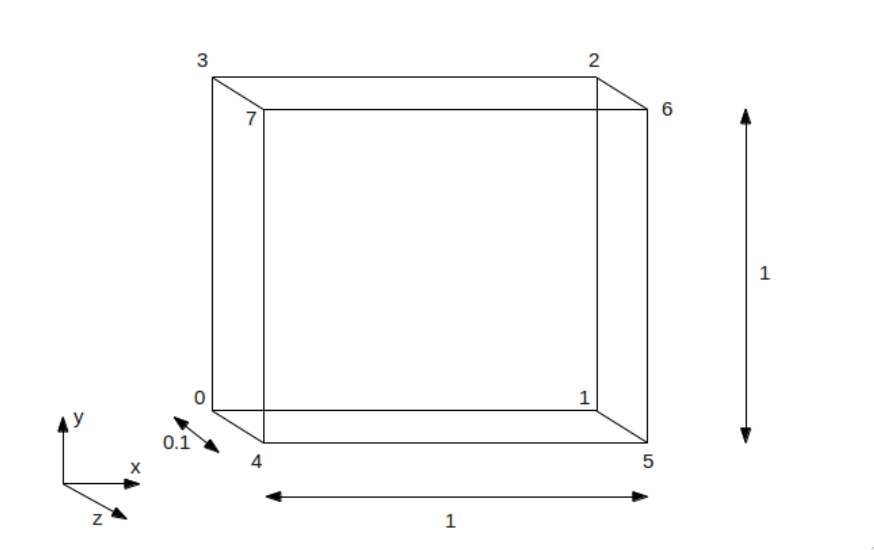
\includegraphics[scale=0.32]{\LocCHtwofig/geometry1.png}
\caption{geomtery points of the lid driven cavity}
\label{geometry}
\end{center}  
\end{figure}
 
\section{blockMeshDict} 
\flushleft Note that in openFoam to create a 2-D geometry you need to give a unit cell thickness in the Z axis. Now in order to create a new geomtry file open a new folder in destop and rename it a “blockMeshDict”. 
\flushleft A blockMeshDict file basically has the following parts:

\begin{itemize}
\item Foam File details
\item vertices
\item blocks
\item edges
\item boundary
\item mergepatchpairs
\end{itemize}

\flushleft Note that the line convertToMeter gives unit in which the geomtery is drawn. For example, as we are drawing the geomtery in meters for this problem we will keep convertToMeters as 1. Now after opening the new blockMeshDict file created in the desktop copy the lines from initial Foam File till convertToMeters from the old file and paste it. After this type vertices and then you can give the X, Y and Z co-ordinates of the boundary as shown below:

\begin{figure}[ht]  
\begin{center}  
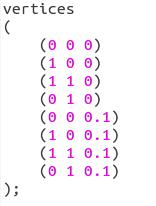
\includegraphics[scale=0.66]{\LocCHtwofig/vertices.png}
\caption{coordinates of boundary geomtery points of the lid driven cavity}
\label{vertices}
\end{center}  
\end{figure}

\flushleft Then type block, inside which you give the details of the boundary co-ordinates along with the number of mesh divisions in X, Y and Z direction in the following way, fig \ref{blocks}:

\begin{figure}[ht]  
\begin{center}  
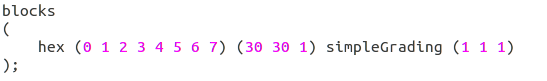
\includegraphics[scale=0.66]{\LocCHtwofig/blocks.png}
\caption{block details of the geomtery}
\label{blocks}
\end{center}  
\end{figure}

\flushleft Here hex represents hexahedral block and the number next to that gives the names of the points at the boundary in clock-wise direction to form a block. Note that for more than one blocks the number of points would be more. The number of grid points can be modified as per requirement. For this problem we have used a 2-D mesh having 30x30 divisions and unit dept. Now since we have all straight edges in this geometry, we will keep the egdes empty.

\begin{figure}[ht]  
\begin{center}  
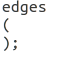
\includegraphics[scale=0.66]{\LocCHtwofig/edges.png}
\caption{edge details of the geomtery}
\label{edges}
\end{center}  
\end{figure}
\vspace{2cm}
\flushleft Next we give the details of the boundary. In the geometry we can see the following boundary conditions,as shown in fig \ref{boundary}:
\begin{itemize}
  \item moving wall
  \item fixed wall
  \item front and back
\end{itemize}
\begin{figure}[ht]  
\begin{center}  
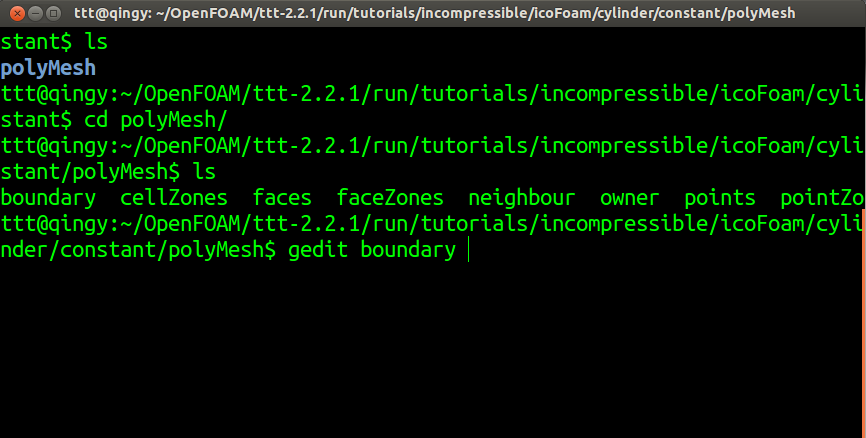
\includegraphics[scale=0.45]{\LocCHtwofig/boundary.png}
\caption{boundary names of the geomtery}
\label{boundary}
\end{center}  
\end{figure}
\flushleft where it has a top moving wall and three fixed wall. The front and back faces are kept empty as this is a 2-D problem. 
\vspace{10cm}
\flushleft Now in the blockMeshDict file you can type the boundary as shown in fig \ref{boundary_name}:
\begin{figure}[ht]  
\begin{center}  
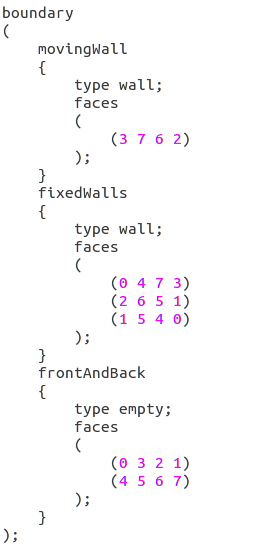
\includegraphics[scale=0.66]{\LocCHtwofig/boundary_name.png}
\caption{boundary details of the geomtery}
\label{boundary_name}
\end{center}  
\end{figure}


\flushleft Here within the boundary names enter the type of boundary used and  then faces, giving the points of the block forming a particular boundary. Note that you should be very careful while writing the order of the points. The order should be such that if you place a folded palm on the surface of a boundary the thumb should be pointing normal to the surface and the fingers should be folded such that they make a curl in clockwise or anti-clockwise direction. Note that you should use either clockwise or anti-clockwise convention throughout the file and but not both. Also you should be very careful regarding openning and closing of brackets in this file.

\flushleft After this$,$ in a new line type mergePatchPairs. Since in this problem we do not have to merge any patches we will keep this empty$,$ fig \ref{merge}.
\vspace{0.32cm}
\begin{figure}[ht]  
\begin{center}  
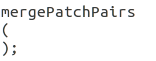
\includegraphics[scale=0.66]{\LocCHtwofig/merge.png}
\caption{merge patch details of the geomtery}
\label{merge}
\end{center}  
\end{figure}

\flushleft Note that two “P”'s are capital here.
\flushleft After completing writing this file save it and close this file. Thus you have learned ho wto create a geomtery file.
\flushleft Now go back to the command terminal and type the following twice to go back to cavity folder:

\center \textbf{cd ..} 

\flushleft Next you can mesh this geomtry by typing blockMesh in the command terminal. After this you can view the geometry by opening paraview. For this type paraFoam in the command terminal and press $<enter>$.
\flushleft In the paraview window press Apply button on the left hand side of the Object Inspector Menu to
view the Geometry, as shown in the fig \ref{paraview1}:
\begin{figure}[ht]  
\begin{center}  
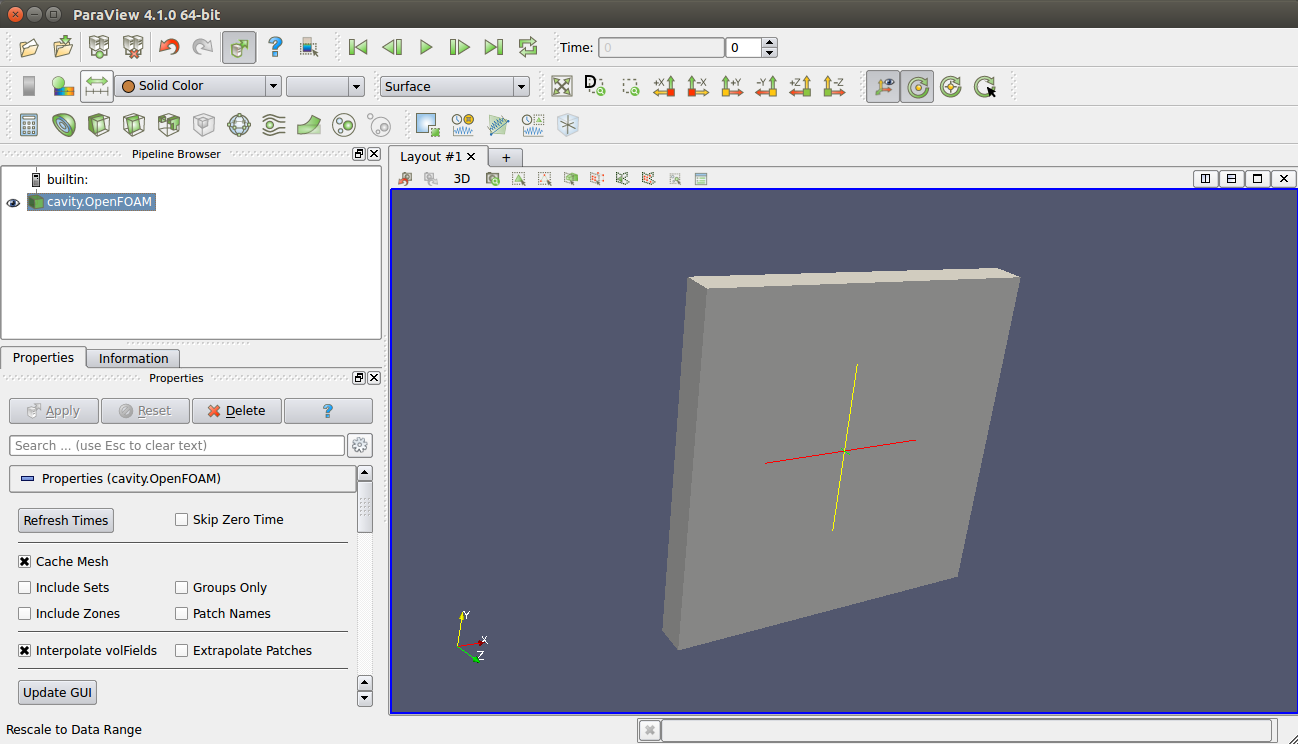
\includegraphics[scale=0.32]{\LocCHtwofig/paraview1.png}
\caption{Paraview window showing the 2-D geometry}
\label{paraview1}
\end{center}  
\end{figure}

\flushleft As you as learned in the previous chapter, you can use different feature in the paraview window to check the details of the geometry.
